\chapter{Results}
\label{chap:Results}

In this chapter, we will present the results obtained from our project. 
Firstly, we will demonstrate how the automation routine enhanced the research experiments. 
Next, we will discuss the validation of the classification results. 
Finally, we will showcase the performance of the implemented controller algorithms.

\section{Automation routine}
\label{sec:automation_routine}

The automated experiment routine is capable of acquiring a significantly more precise and extensive amount of data than what can be achieved by a human. 
With the save data by streaming in saving thread \ref{subsec:save_thread}, we achieved less program memory during the experiment and, specially, safety for not losing the data in case the program fail during an experiment.

Also, most power supplies rely on manual potentiometer adjustment to select the set point, which results in imprecise potential selection by a person and takes some time to achieve the desired voltage.
Moreover, the electrospray phenomena has a known hysteresis, that can be seen in figure \ref{fig:ganan_calvo_fig}, and can perform different results depending on the previous electric potential.
By running a computer routine that automatically sends commands to the power supply and pump machine we can achieve faster and more reliable experiment data points.

The visual interface for the user, seen in figure \ref{fig:multi_class_exp1}, shows all the important sensor data and signal analysis that can be interesting to the operator in real time, serving as a supervisory system.

\begin{figure}[H]
    \center
    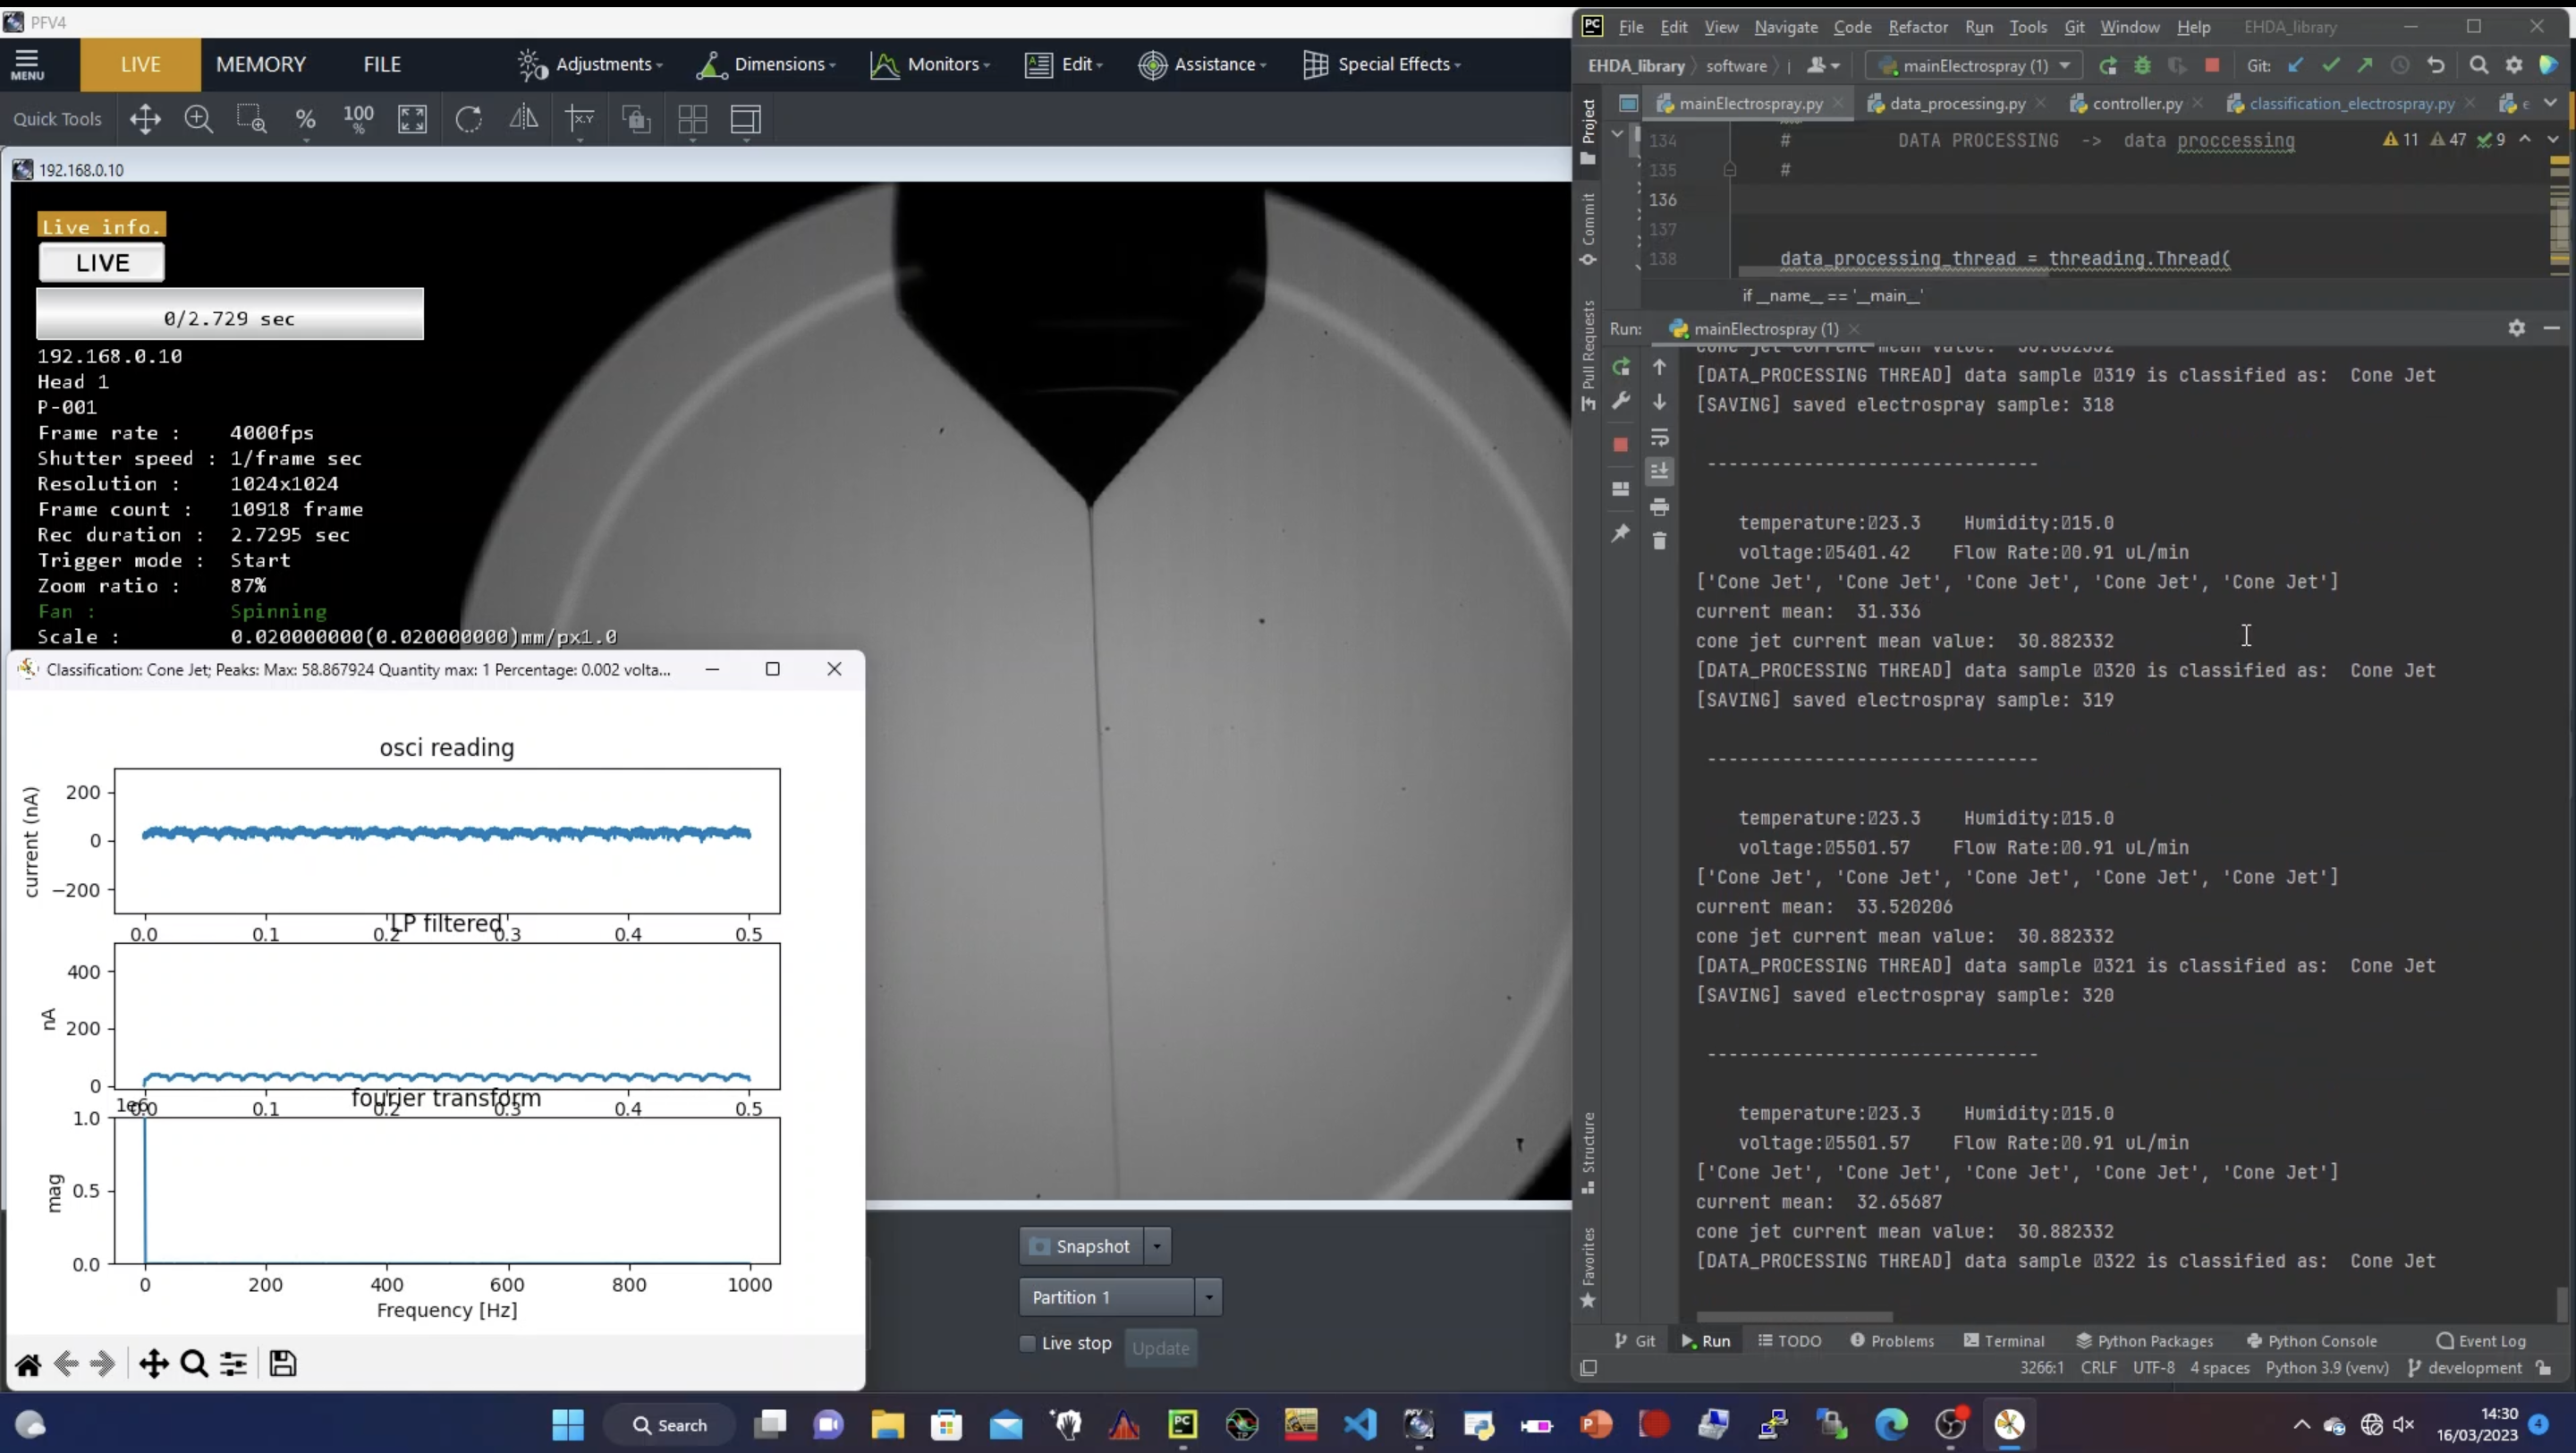
\includegraphics[width=16cm]{Figuras/19:03/axs1.png}
    \caption{Print screen of the window shows user interface during the experiment.
        We can see the image generated by the camera in the background.
        The routine code running in pycharm software on the right side.
        And also real time signal plottings of the current data on the left side.}
        \label{fig:multi_class_exp1}
\end{figure}


\section{Classification}
\label{sec:classification_results}

The classification results in our algorithm implemented as described in section \ref{sec:section_classification} showed good accuracy for all the classifications described in section \ref{sec:spraying_modes_subsec}.
Nevertheless, the multi jet classification made by a current value factor of 1.14 above the cone jet is just effective for pure ethanol, liquid used in all this project.

Even if the multi jet classification just works for pure ethanol, the data saved with correct classification in ethanol can be used to extract any other signal information about the multi jet or to train a black box classification algorithm.

We will categorize our classification results into two main groups - the step routine and the map routine. These two routines have showed valuable insights and comprehensible results of the electrospraying process.


\subsection{Step Sequence}
\label{subsec:step_results}

Our first classification results were made exploring the voltage ranges. 
For that, we fixed a flow rate to 0.7 uL/min. and ran a step routine as defined in \ref{subsec:step_routine}. 
The figure \ref{fig:step_class} shows three graphs. 

The first shows the controller output signal as an input voltage of the process. As it is a step routine we implemented a increasing voltage with steps of sizes 50V and time between each step of 5 seconds. The voltage range is between 3K~10K Volts.

The second is the raw output data collected by the oscilloscope in \emph{data\_acquisition\_thread()}. 
The sampling rate is 10KHz. Therefore, this experiment of 700s has 7 Million data points just of current data. 
This is an example of how scalable the data collected can be depending on the experiment time. This will be even more noticeable in mapping experiments.

The Third graph is the same data as the second after the classification procedure done by \emph{data\_processing\_thread()}. 


\begin{figure}[H]
    \center
    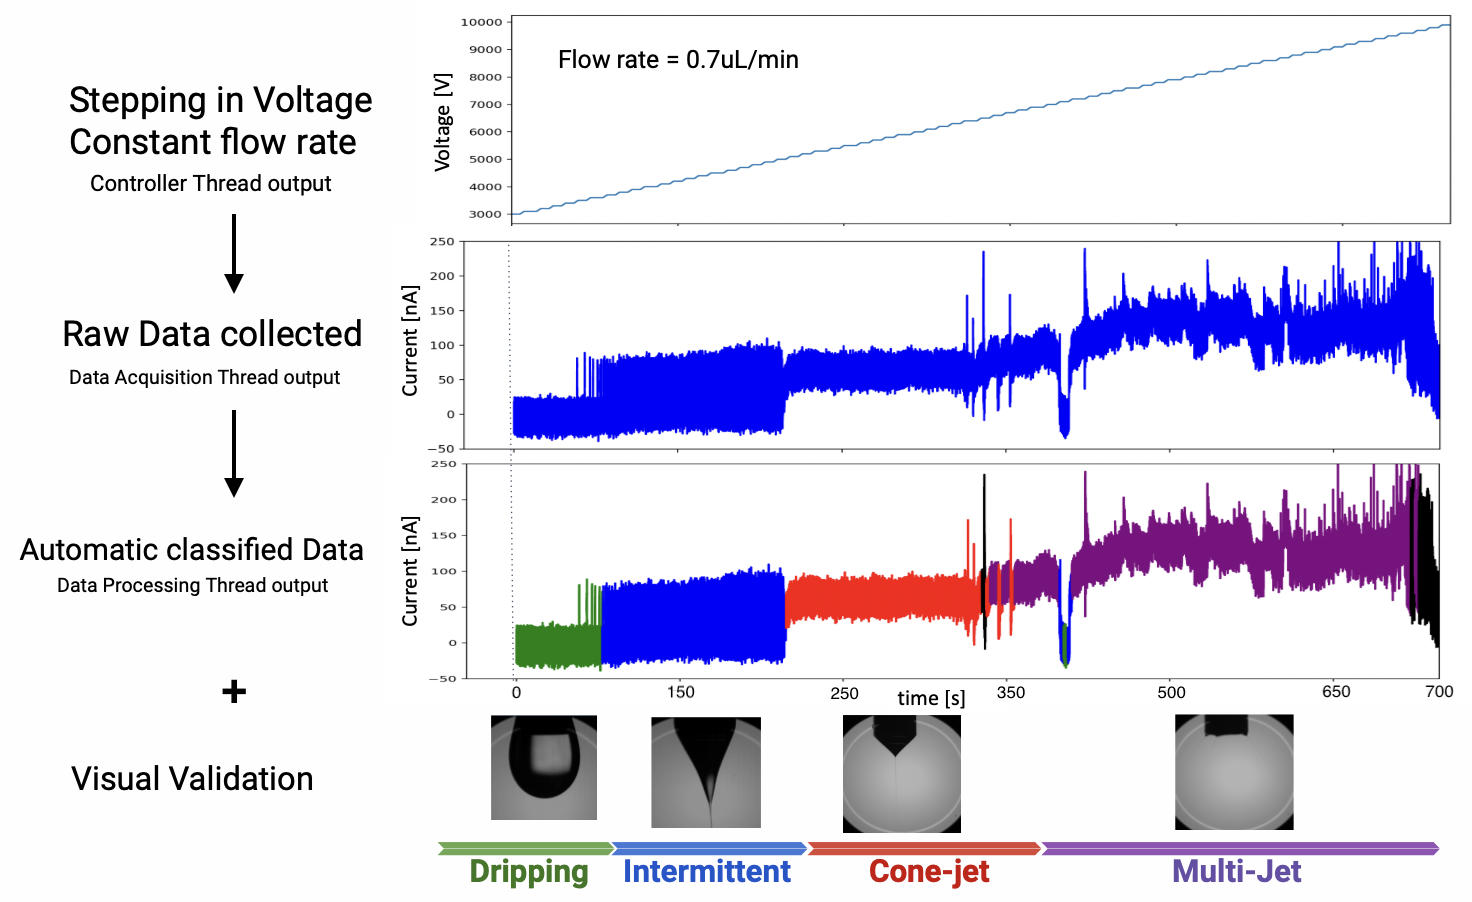
\includegraphics[width=16cm]{Figuras/may/step_class.png}
    \caption{Automatic electrospray classification through the step routine.}
    \label{fig:step_class}
\end{figure}

The graph of voltage scan has a common shape for different liquids and parameters. After having familiarity with it, is even possible to classify the spraying modes by visual analysis. 

For example, dripping mode has a current mean of 0V. The Intermittent state has a high variation of values that can be seen by the increased thickness on the graph. The Cone jet is a thinner graph because of its constant signal. Multi Jet  has the same shape as Cone jet but with a higher mean value. Corona sparks are not showed in the graph because its discharges has a high current value above the axis limits.



\subsection{Map Sequence}
\label{subsec:map_results}

For validation with literature and also to expose the benefits of the automated routine and classification, the map sequence proof itself the best result of this work.

    Initially, for better understand pure ethanol classification regions through voltage and flow rate ranges, I made a manual map seen in figure \ref{fig:stability_1}.

    \begin{figure}[H]
        \center
        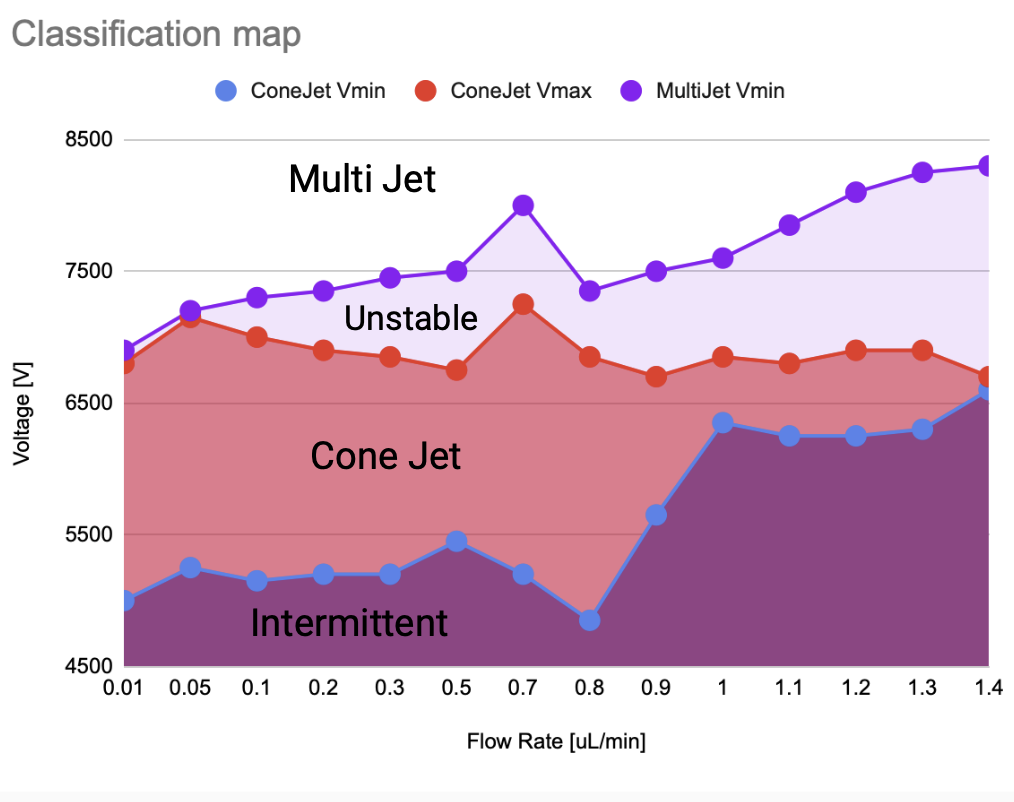
\includegraphics[width=12cm]{Figuras/regions.png}
        \label{fig:stability_1}
        \caption{Experimental spraying modes regions of pure ethanol}
    \end{figure}


    In order to validate our automatic classification, experiments were made comparing both visual and automatic stability island on the same experiment.
    Figure \ref{fig:stability_2} shows that automatic stable cone jet region could be identified in the same region as visually seen by the high speed camera (data acquired manually).

        \begin{figure}[H]
            \center
            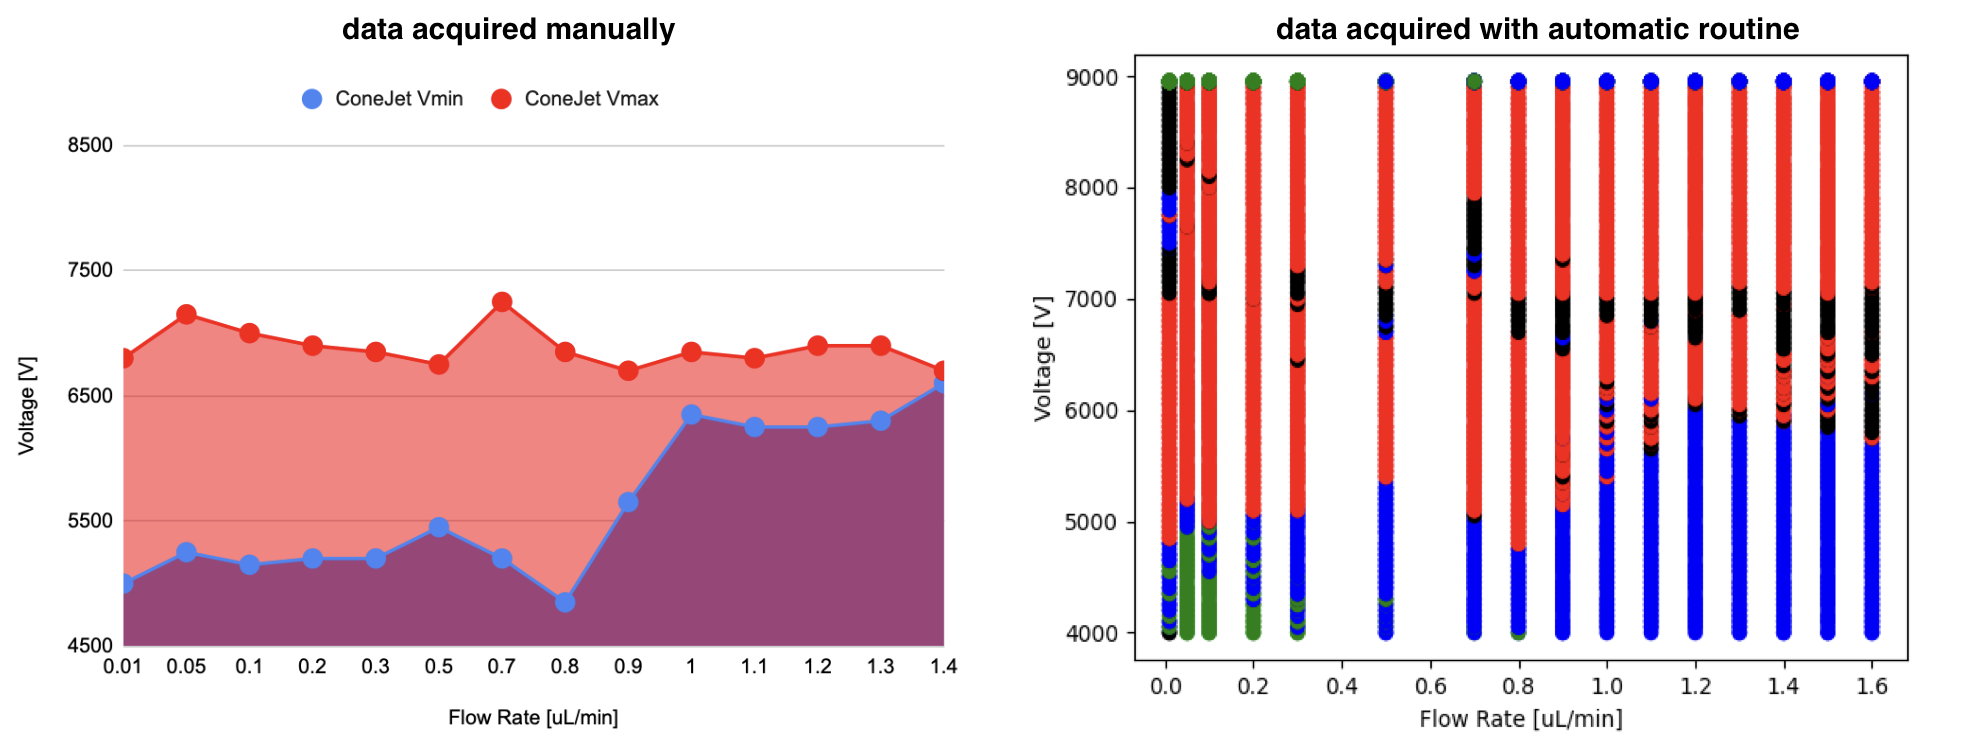
\includegraphics[width=16cm]{Figuras/april/manual_stability_island.png}
            \caption{Cone jet stability region for pure ethanol experiment 1}
            \label{fig:stability_2}
        \end{figure}


    With the development of a Multi Jet classification using the logic explained in section \ref{sec:section_classification}, I repeated the same experiment as shown in Figure \ref{fig:stability_6}.


        \begin{figure}[H]
            \center
            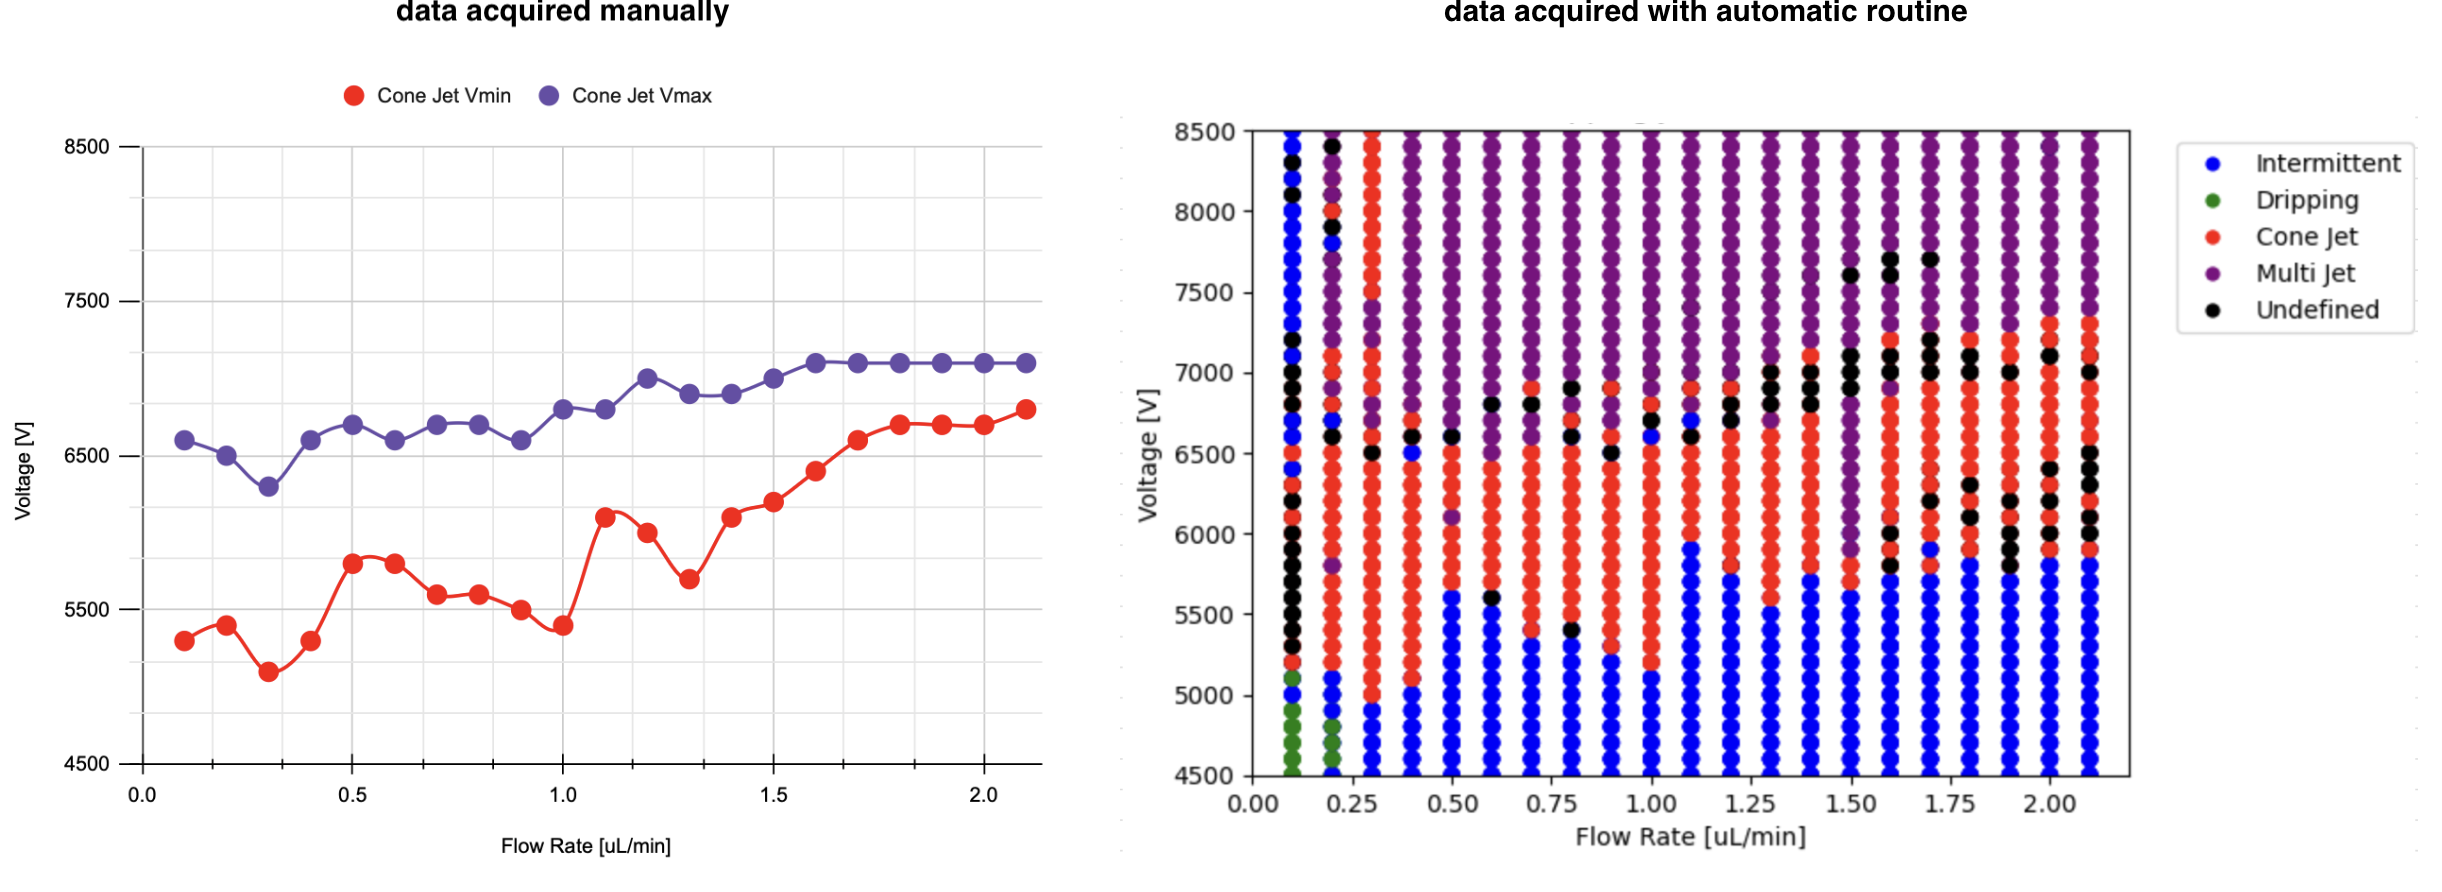
\includegraphics[width=18cm]{Figuras/april/map_third.png}
            \caption{Cone jet stability region for pure ethanol experiment 2}
            \label{fig:stability_6}
        \end{figure}


    \subsubsection{Non-dimensional axis}

    To have a better comparison with literature, specifically the Gañán-Calvo\cite{gananCalvo} stability islands showed in figure \ref{fig:ganan_calvo_fig}, with a visual juxtaposition of the shapes, we displayed in figure \ref{fig:stability_8} the data using the non-dimensional numbers used in his work\cite{gananCalvo}.

        \begin{figure}[H]
            \center
            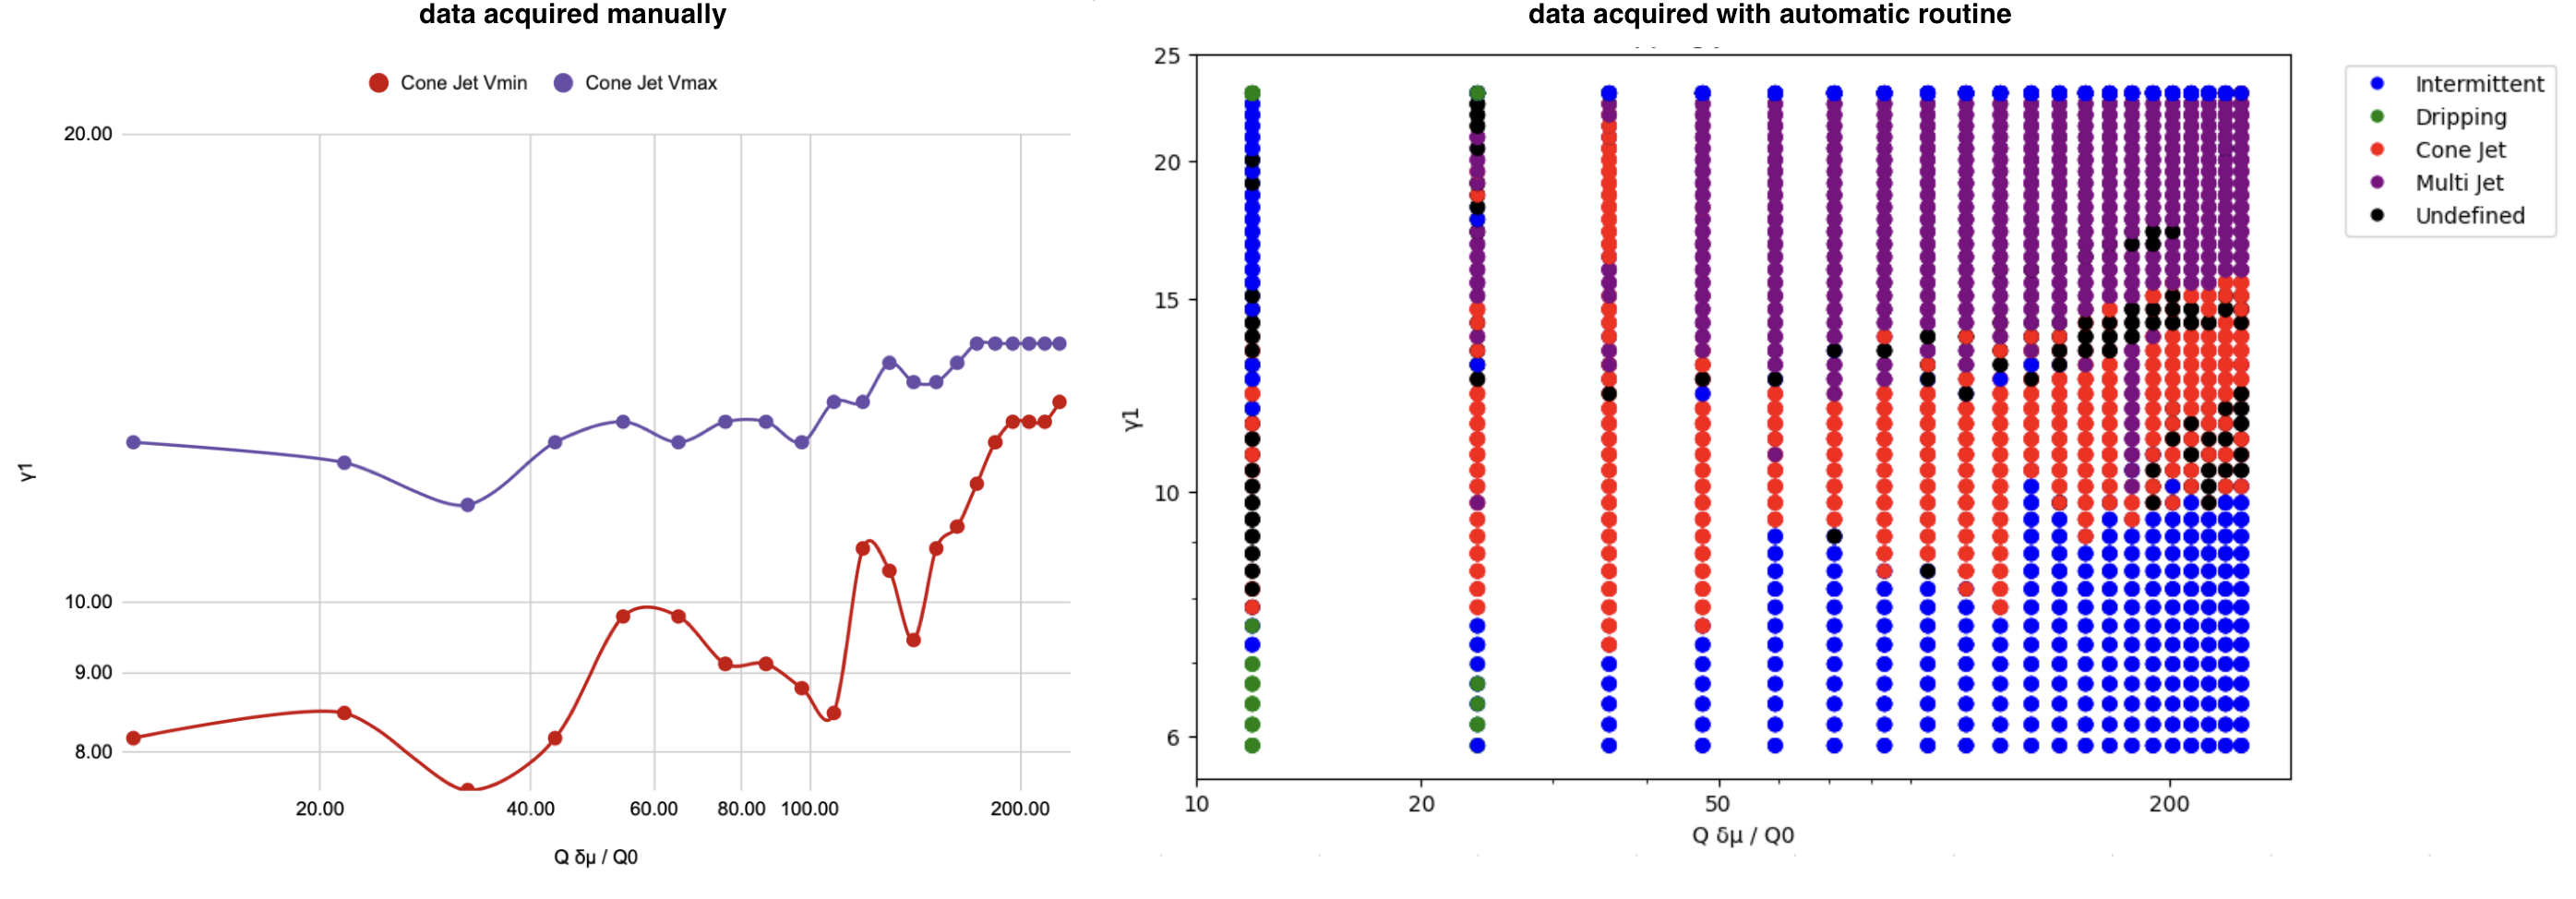
\includegraphics[width=18cm]{Figuras/april/manual_au_1.png}
            \caption{Cone jet island manual experiment 4}
            \label{fig:stability_8}
        \end{figure}

    The results of mapping experiment corresponded visual, literature and automatic regions of classification, giving authentication to our method.


\section{Controller}
\label{sec:controller_results}

    The results of the classification process were favorable for experiment automation, however, the inaccuracy of the classification by statistical methods, specially the Multi Jet\ref{subsec:Multi Jet}, limited the development of a complete control project.
    Together with the amount of variables that need to be syntonized makes it hard to stabilize in a desired mode.

    Even with all those problems we could implement a simple controller project, described in \ref{sec:control_model}, that validated the efforts of remodeling all software into a closed loop control model.
    
    The controller not only stabilized in Cone Jet mode, but also could reject perturbation, as seen in Figure \ref{fig:control_results}, where I manually changed the flow rate.
    First graph shows current acquired. It starts as intermittent state, with an oscillating signal. We can validate this with the blue colored sample on the third graph representing its automatic classification. 
    The second graph shows the controller actuating increasing the voltage to achieve a stable cone jet mode.
    After a period of time in cone jet, I manually increased the flow rate, serving as a perturbation of the system, and we can see that the effect of that was to return to intermittent state with the oscillating signal. The controller again, actuate increasing the voltage to reach the cone jet stability island. 
    This procedure was repeated after some seconds of stabilization in cone jet, increasing again the flow rate manually, and we can see the system automatically adjusting the voltage.
        \begin{figure}[H]
            \center
            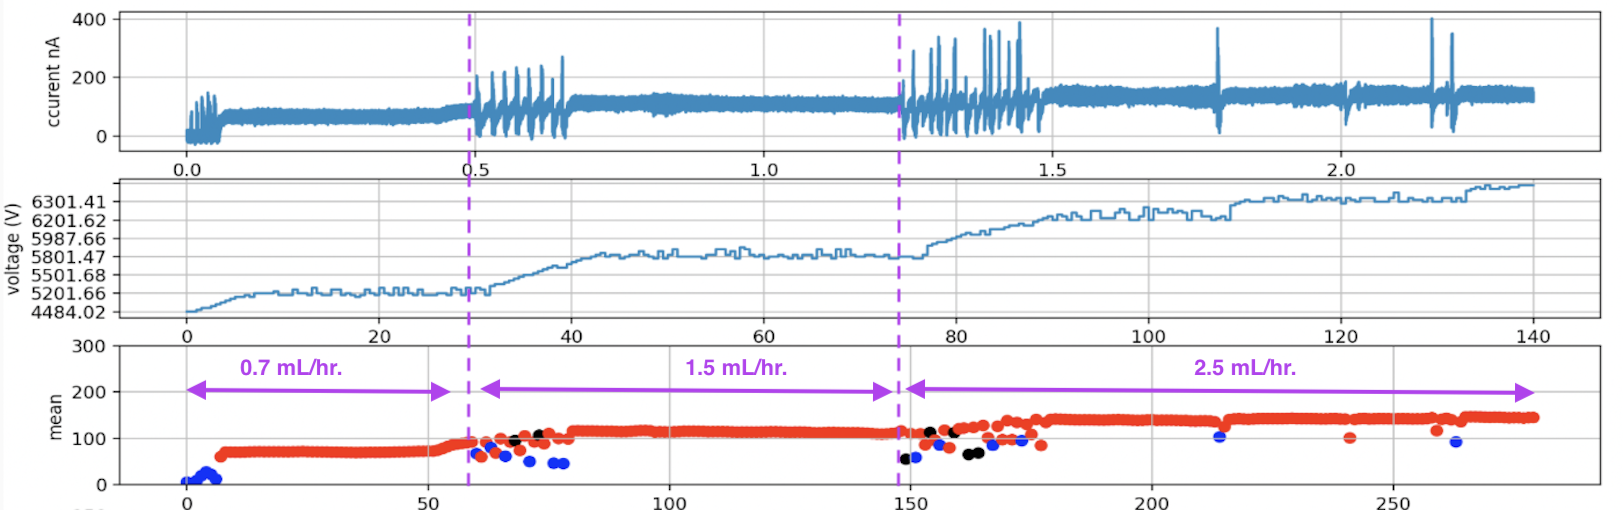
\includegraphics[width=16cm]{Figuras/19:03/control_first_results.png}
            \caption{Simple controller validation experiment. For this experiment we waited the system to stabilize in the desired spraying mode. After that we made a perturbation test changing the flow rate. The classification legend follows the same color reference in all project.}
            \label{fig:control_results}
        \end{figure}

    After 200s of experiment we had some breaks up of the cone jet into a droplet and stabilized again. This is represented by the peak values in current signal. The classification correctly identified as intermittent, seen as blue dots in the third graph, and the controller reacted increasing the voltage, in a situation that can be considered as noise. A filter can be applied in a more complex controller project to avoid this.
    


\section{Chapter conclusion}

In this chapter we exposed the results of this project. The automatic routine, real time classification and control were all achieved and implemented. However, they can all be improved. In the next Chapter I will conclude this document with discussions about the results and proposal of continuation.


\clearpage